\documentclass[tikz, border=15pt]{standalone}
\usepackage{tikz}
\usetikzlibrary{calc, arrows.meta, patterns}

\definecolor{steel}{HTML}{708090}
\definecolor{darksteel}{HTML}{4A5568}
\definecolor{pistonred}{HTML}{E53E3E}
\definecolor{fluidblue}{HTML}{3182CE}
\definecolor{fluidlight}{HTML}{90CDF4}
\definecolor{chamberbg}{HTML}{EBF8FF}

\begin{document}
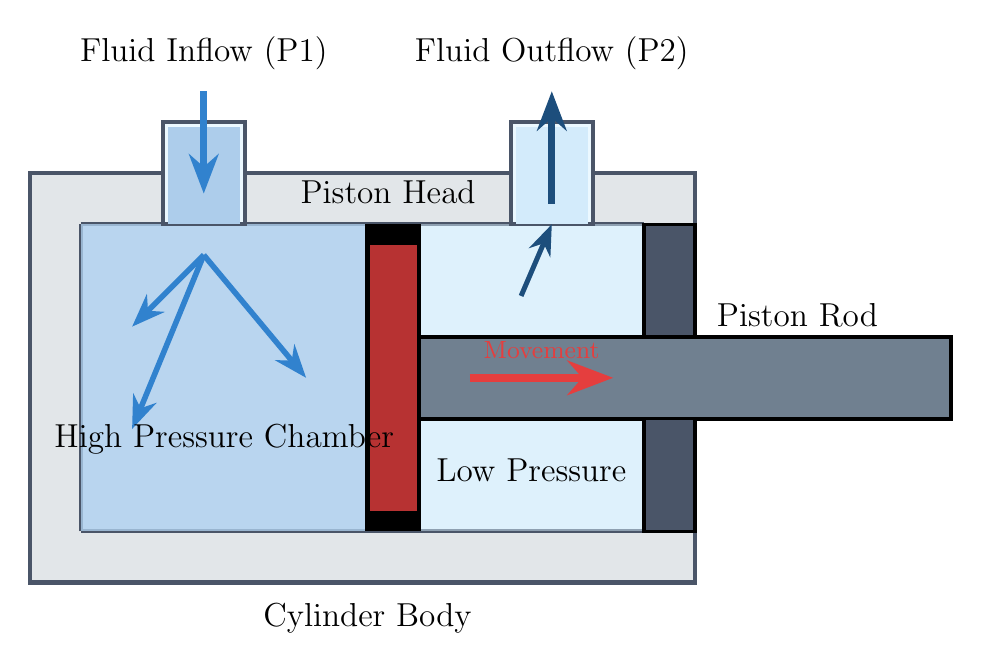
\begin{tikzpicture}[
    scale=1.3,
    >=Stealth,
    line width=1.2pt,
    font=\sffamily\bfseries
]

    % Cylinder Housing Cross Section (Outer Wall)
    \fill[steel!20, draw=darksteel, line width=1.5pt] (-4.5, -2.0) rectangle (2.0, 2.0);
    % Hollow Interior
    \fill[chamberbg] (-4.0, -1.5) rectangle (1.5, 1.5);
    \draw[darksteel, line width=1.5pt] (-4.0, -1.5) -- (1.5, -1.5);
    \draw[darksteel, line width=1.5pt] (-4.0, 1.5) -- (1.5, 1.5);
    \draw[darksteel, line width=1.5pt] (-4.0, -1.5) -- (-4.0, 1.5); % Left cap

    % High-pressure Fluid in Left Chamber
    \fill[fluidblue!40, opacity=0.8] (-4.0, -1.5) rectangle (-1.2, 1.5);

    % Low-pressure / Exhaust Fluid in Right Chamber
    \fill[fluidlight!40, opacity=0.5] (-0.7, -1.5) rectangle (1.5, 1.5);

    % Piston Head
    \fill[pistonred!80!black, draw=black, line width=1.5pt] (-1.2, -1.48) rectangle (-0.7, 1.48);
    % Seals on Piston
    \fill[black] (-1.2, 1.3) rectangle (-0.7, 1.48);
    \fill[black] (-1.2, -1.48) rectangle (-0.7, -1.3);

    % Piston Rod
    \fill[steel, draw=black, line width=1.5pt] (-0.7, -0.4) rectangle (4.5, 0.4);
    % Rod Guide / Seals on Right Cylinder Cap
    \fill[darksteel, draw=black] (1.5, -1.5) rectangle (2.0, -0.4);
    \fill[darksteel, draw=black] (1.5, 0.4) rectangle (2.0, 1.5);

    % Fluid Ports
    % Left Port (Inflow)
    \fill[chamberbg, draw=darksteel, line width=1.5pt] (-3.2, 1.5) rectangle (-2.4, 2.5);
    \fill[fluidblue!40] (-3.15, 1.5) rectangle (-2.45, 2.45);
    % Right Port (Outflow)
    \fill[chamberbg, draw=darksteel, line width=1.5pt] (0.2, 1.5) rectangle (1.0, 2.5);
    \fill[fluidlight!40] (0.25, 1.5) rectangle (0.95, 2.45);

    % Fluid Flow Arrows
    % Inflow arrow left
    \draw[->, line width=2.5pt, fluidblue] (-2.8, 2.8) -- (-2.8, 1.8);
    \draw[->, line width=2pt, fluidblue] (-2.8, 1.2) -- (-3.5, 0.5);
    \draw[->, line width=2pt, fluidblue] (-2.8, 1.2) -- (-3.5, -0.5);
    \draw[->, line width=2pt, fluidblue] (-2.8, 1.2) -- (-1.8, 0);

    % Outflow arrow right
    \draw[->, line width=2.5pt, fluidblue!60!black] (0.6, 1.7) -- (0.6, 2.8);
    \draw[->, line width=1.8pt, fluidblue!60!black] (0.3, 0.8) -- (0.6, 1.5);

    % Piston Movement Arrow (Extending to right)
    \draw[->, line width=3pt, pistonred] (-0.2, 0) -- (1.2, 0) node[midway, above=2pt, font=\small] {Movement};

    % Labels & Annotations
    \node[above, font=\large] at (-2.8, 2.9) {Fluid Inflow (P1)};
    \node[above, font=\large] at (0.6, 2.9) {Fluid Outflow (P2)};
    \node[font=\large] at (-2.6, -0.6) {High Pressure Chamber};
    \node[font=\large] at (0.4, -0.9) {Low Pressure};
    \node[above, font=\large] at (-1.0, 1.6) {Piston Head};
    \node[above, font=\large] at (3.0, 0.4) {Piston Rod};
    \node[below, font=\large] at (-1.2, -2.1) {Cylinder Body};

\end{tikzpicture}
\end{document}
